\section{Evaluation}
    \paragraph{}
    In this section, we will draw out conclusions from the models trained and compare them. As seen in section 3.3 and 3.4, we can conclude that our best model is CNN with 72.37\% accuracy.
    
    To further evaluate the models, we plotted their confusion matrix and classification report.
    
    \subsection{Confusion Matrix}
    \begin{figure}[H]
        \centering
        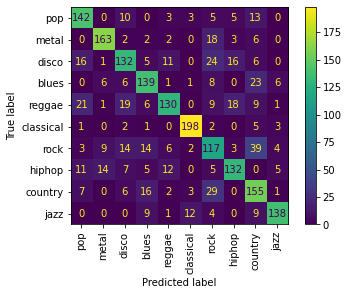
\includegraphics[width=0.35\textwidth]{images/cnn_matrix.png} 
        \caption{CNN confusion matrix}
    \end{figure}

    \begin{figure}[H]
        \centering
        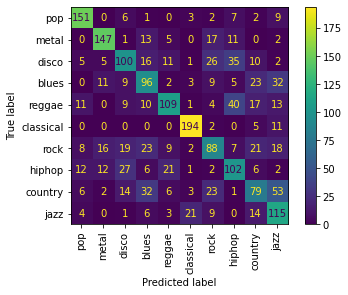
\includegraphics[width=0.35\textwidth]{images/rnn_matrix.png} 
        \caption{RNN confusion matrix}
    \end{figure}  
    
    \paragraph{}
    As we can see, from figure 5 and 6, the CNN made less errors than the RNN. Both has more accurately predicted classical music. Our CNN model misclassified rock as country the most while our RNN model misclassified country as jazz the most.
    
    From the diagonal of both confusion matrix, the CNN model performed way better.
    
    \subsection{Classification Report}
    \begin{figure}[H]
        \centering
        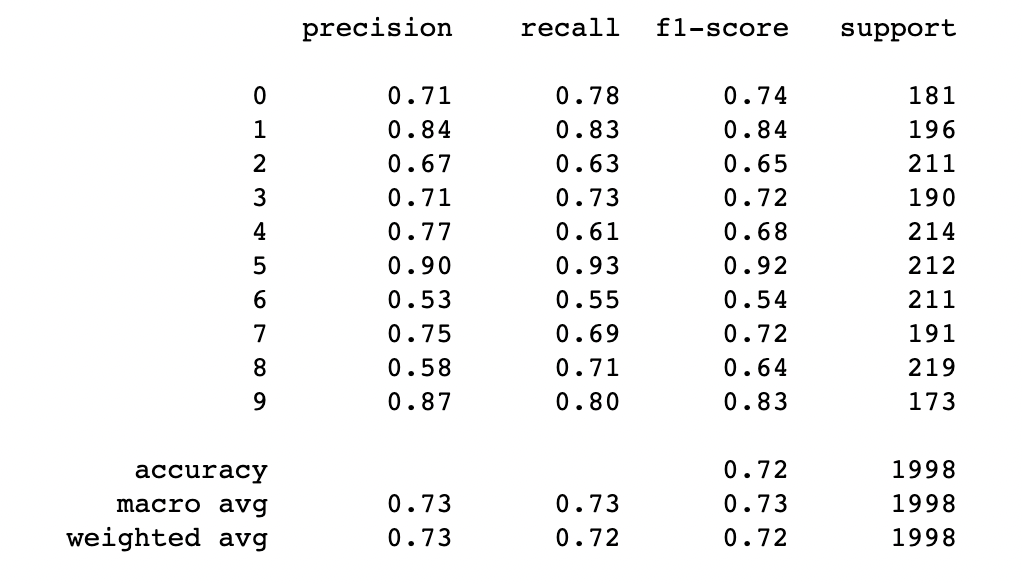
\includegraphics[width=0.4\textwidth]{images/cnn_classification_report.png} 
        \caption{CNN classification report}
    \end{figure}

    \begin{figure}[H]
        \centering
        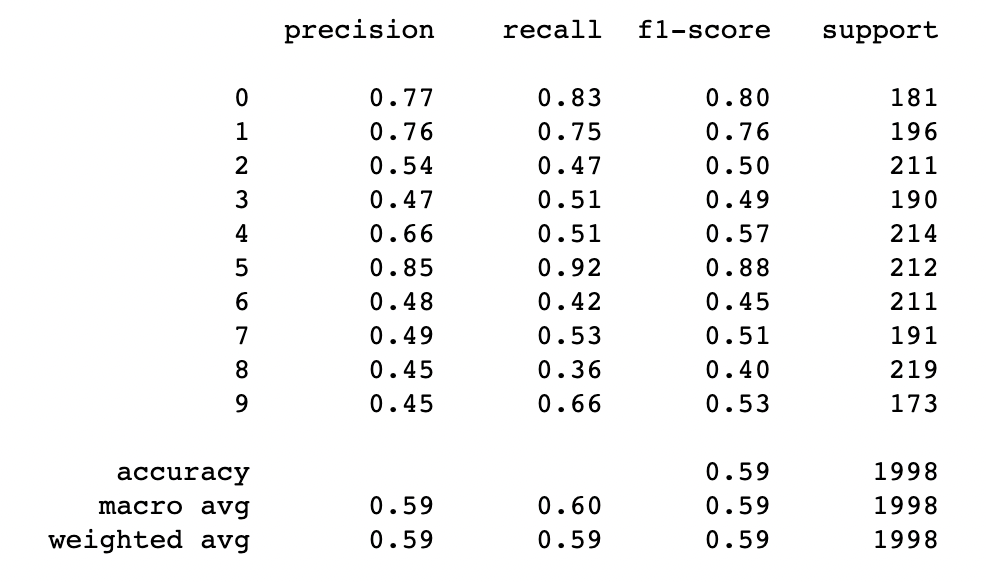
\includegraphics[width=0.4\textwidth]{images/rnn_classification_report.png} 
        \caption{RNN classification report}
    \end{figure}
    
    \paragraph{}
    Looking at the classification report from figure 7 and 8, our CNN model have higher precision, recall and f1-score. Our CNN model has on average 0.73 for all three metrics while our RNN model has 0.59, 0.60, 0.59 respectively.
    
    \paragraph{}
    To conclude, the CNN model had better precision and recall than the RNN model.
    
\section{Conclusion}
\paragraph{}
Finally, we are quite satisfied with the accuracies achieved. We were also able to create an interactive way for a user to use our model. The user would be able to copy and paste a YouTube link to the \href{https://github.com/xkaDachi/COMP432_Music_Classification/blob/main/Music%20Classification.ipynb}{jupyter notebook} itself and we would predict its genre with our best model (see figure 9).
\begin{figure}[H]
        \centering
        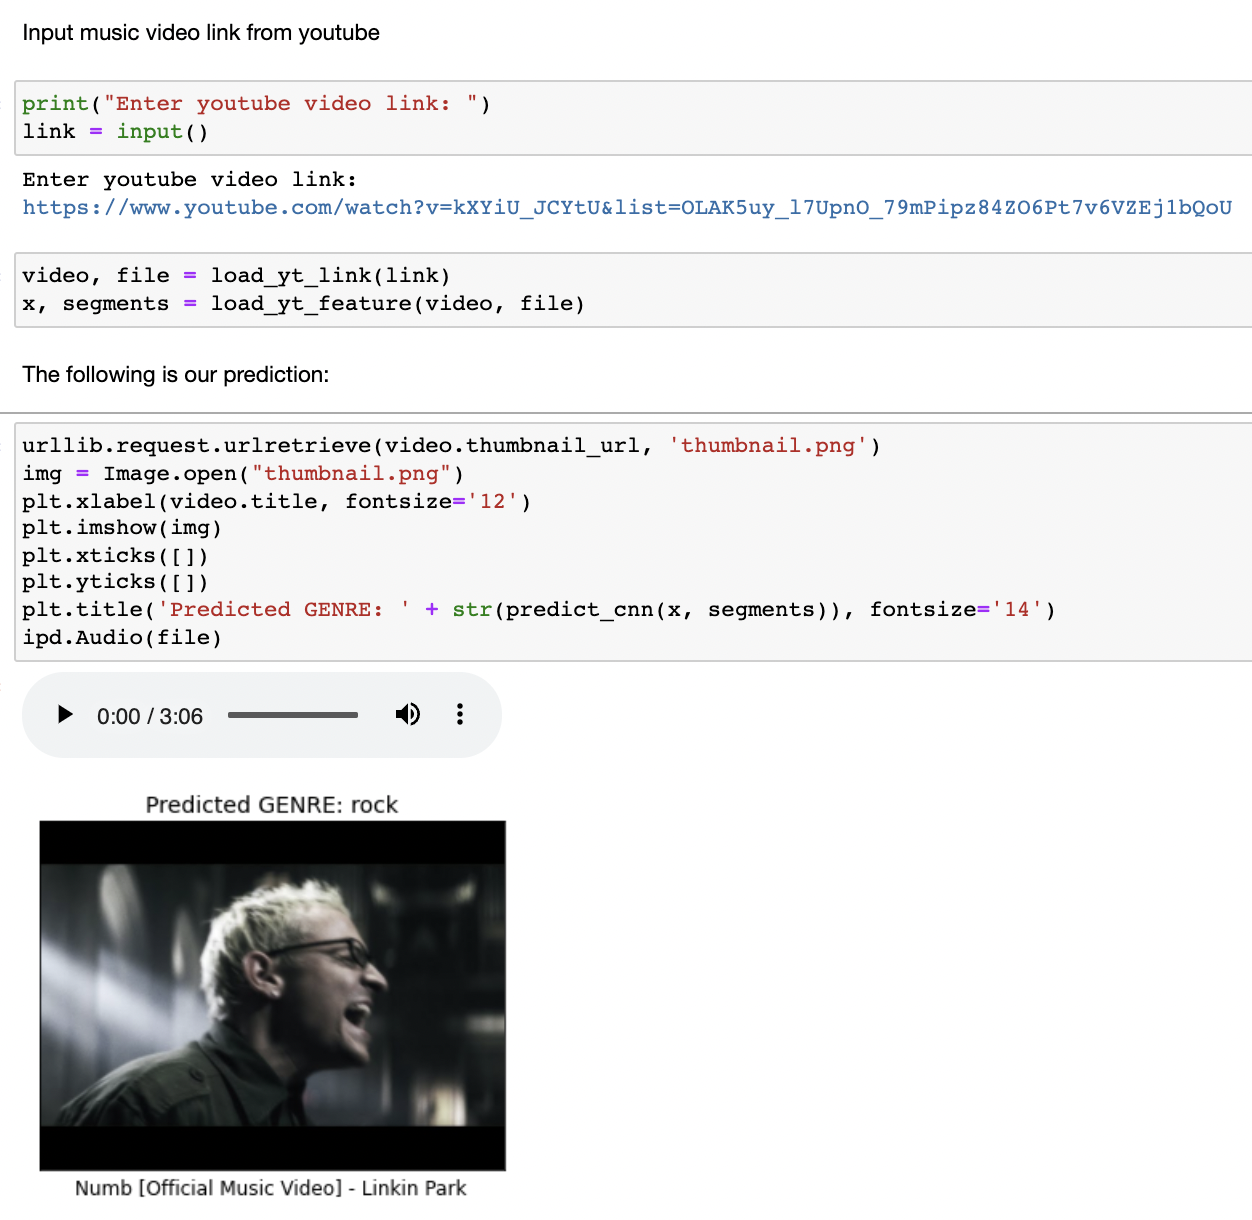
\includegraphics[width=0.4\textwidth]{images/yt_pred.png} 
        \caption{YouTube prediction}
    \end{figure}
\paragraph{}
In the event that we plan to further improve BitByteBeat, we agreed that we would require substantially more training data, both in the form of more genre types as well as overall dataset size. Genres change over time and our dataset currently has old songs. A major improvement would be to update our dataset with more recent songs. 
With this we could classify a larger set of songs more accurately.\\ 

In addition we also discussed the prospect of training it with other models like KNN or adding other audio features like volume, energy, pitch, etc along with the MFCC. We could also try applying feature selection techniques like Principal Component Analysis to identify optimal features to further improve results.\\

We have also looked into switching from the Keras framework of Tensorflow to the PyTorch framework. It could have been pleasant to compare the training speed of the model between the two frameworks and potentially see one of them being faster. It could have been interesting to analyze which model is better through its accuracy and testing between both CNN and RNN models depending on the framework used. \\

That being said, we can only talk about the 'what if' and 'why not' now because of all the knowledge we gained throughout the project. We indeed learned a lot and are very happy to have reached this level of completion. More specifically, it was really fun to try out our model on different YouTube songs and have a good laugh about it. It was a great introduction to Machine Learning for all of us!
